
\begin{figure}[t]
    \centering
    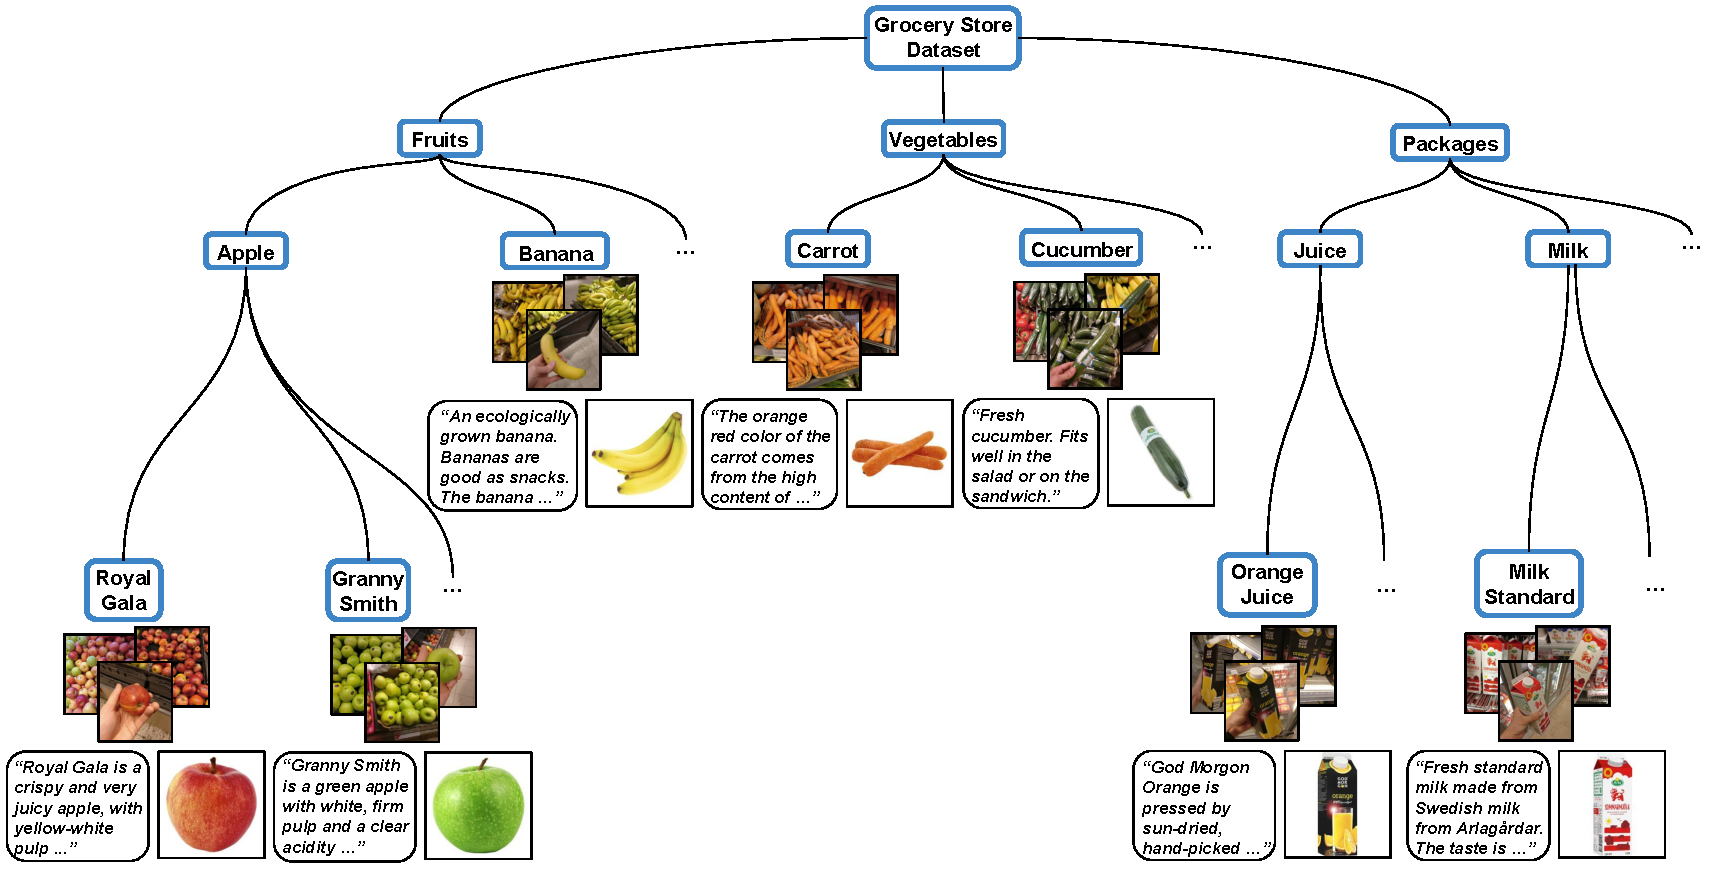
\includegraphics[width=\textwidth]{PaperB/figures_and_tables/dataset_figures/dataset_figure_new.pdf} %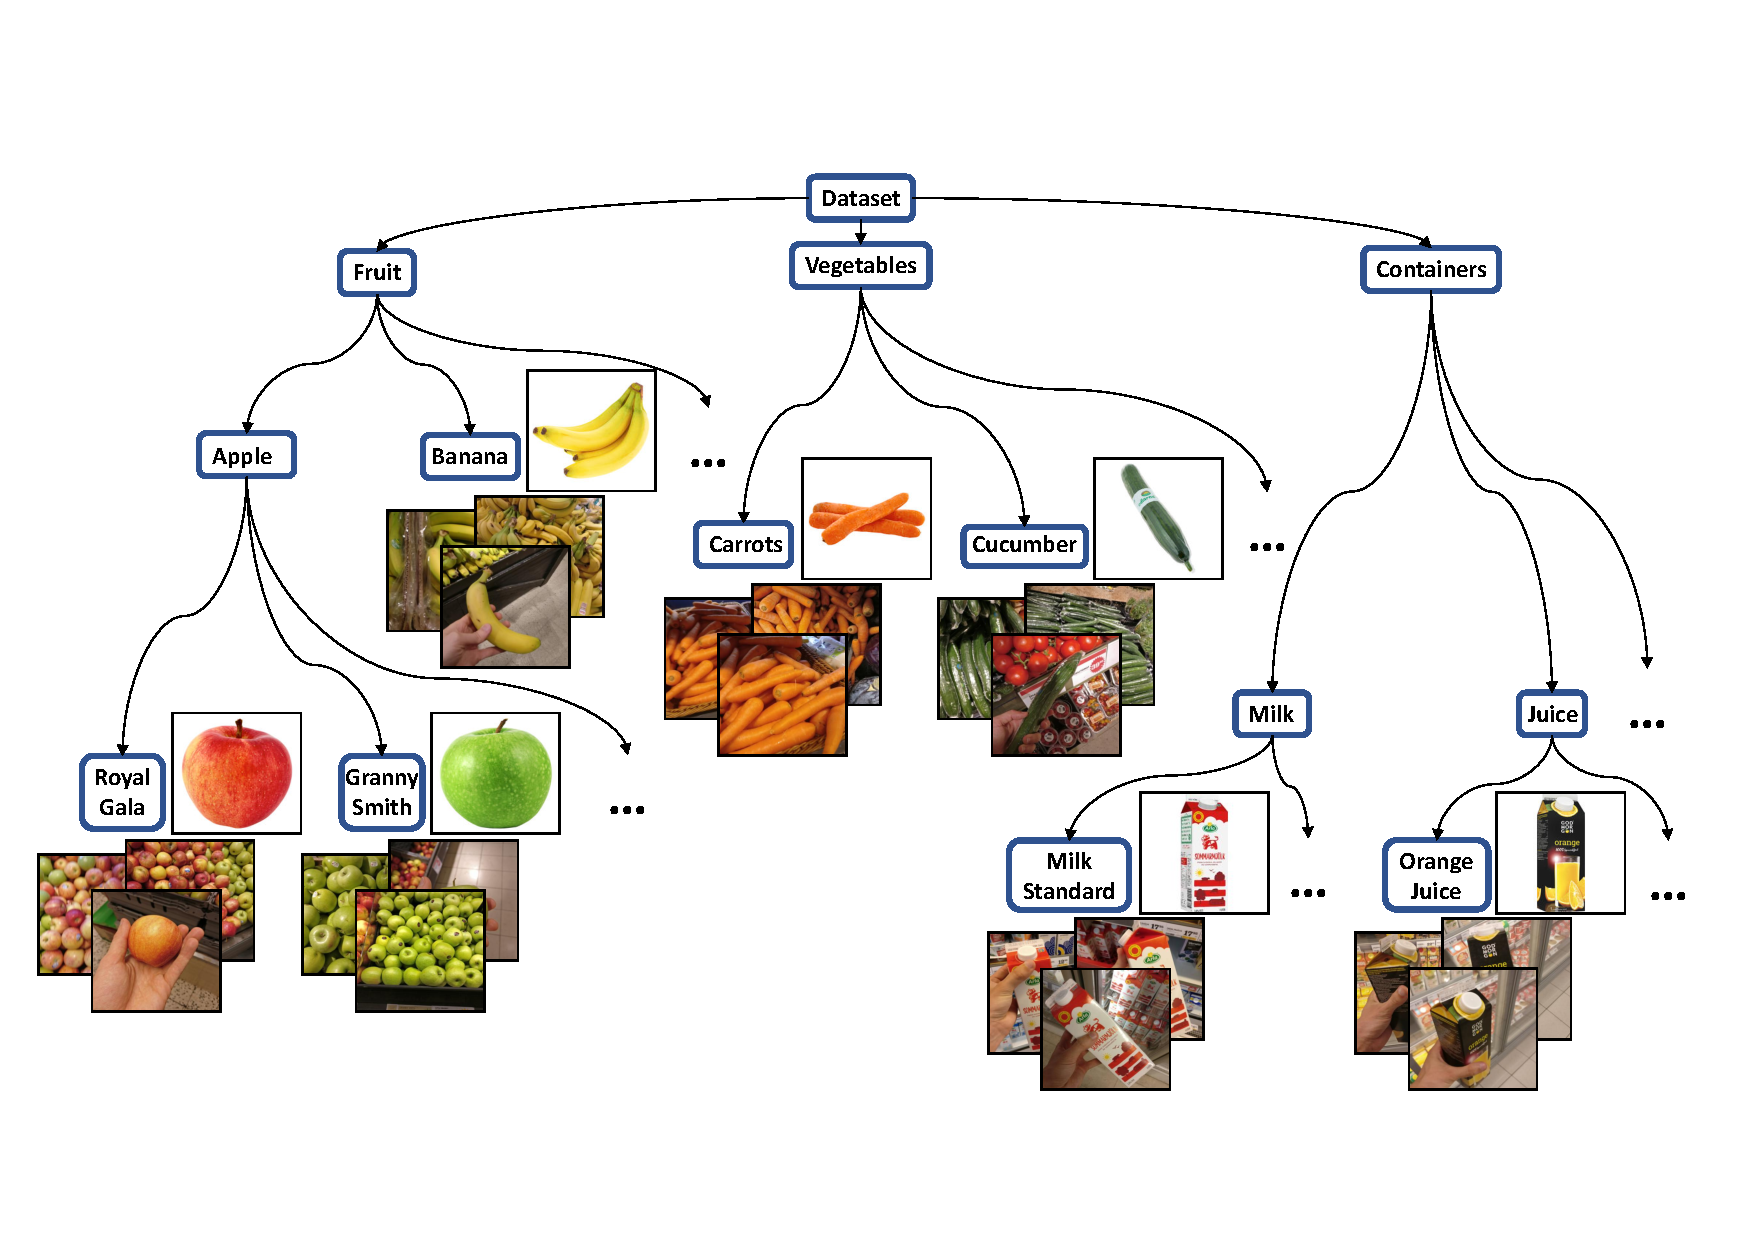
\includegraphics[width=0.95\textwidth]{dataset_figures/intro.pdf}
    \vspace{-2mm}
    \caption{Illustration of the hierarchical class structure of the dataset. First, the classes are divided by their grocery item type, i.e., \textit{Fruits}, \textit{Vegetables}, and \textit{Packages}, followed by a separating the items into coarse-grained classes, e.g., \textit{Apple}, \textit{Carrot}, and \textit{Milk}, and then into fine-grained classes. There are 81 fine-grained classes in total and 46 coarse-grained classes. The figure also shows the iconic image and text description of the items next to the class label.
   }
    \label{fig:examples} 
\end{figure}